\chapter{Data Exploration Visualisation}\
\begin{boxH}
  A \textbf{Dataset} is a \textbf{collection of data}, for example a tabular
  representation made of rows and columns. 
\end{boxH}
The \textbf{size} of the dataset has a \textbf{huge impact} on the choice of
the analyses, for example some algorithms are not suitable for big dataset 
because they are too slow. 

\textbf{Each column} of the dataset represents on attribute or \textbf{feature}
and \textbf{each rows} is a \textbf{different sample}
Each attribute we can be analyzed based on their measurement, attribute
type(numerical or categorical) and domain. To gain some information, starting
from a theoretical distribution we use the min, max, avg, mean value, standard
deviation or mathematical function.

\section{Distribution Visualization}
One of the most common way to represent the distribution of a dataset is the
\textbf{histogram}, that is a graphical representation of the distribution of
data. The range of values are divided into bins, which are basically intervals
of values, and the number of values that fall into each bin is counted. 
\begin{figure}[H]
  \centering
  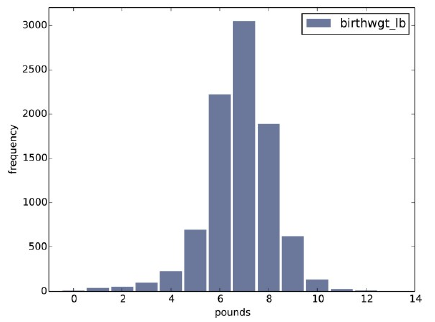
\includegraphics[scale=.60]{images/DataExplVis/hist.png}
  \caption{An example of histogram hat shows the distribution of pound part
  of birth weight}
  \label{fig:hists}
\end{figure}
\subsection{Classification of distribution}
The distribution can be classified as:
\begin{itemize}
  \item \textbf{Discrete probability distribution} if the data is discrete
  \item \textbf{Continuous probability distribution} if the data is continuous
\end{itemize}
\subsection{Probability Mass Function (PMF)}
The PMF is a function that gives the probability that a discrete random
variable is exactly equal to some value. Its typically used for discrete
variables.
\begin{figure}[H]
  \centering
  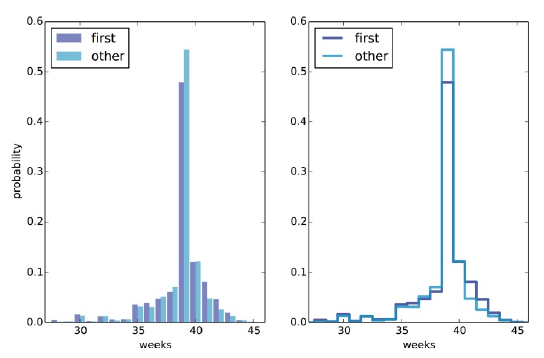
\includegraphics[scale=.60]{images/DataExplVis/pmf.png}
  \caption{An example of PMF}
  \label{fig:pmf}
\end{figure}
This kind of visualization has some limitation, for example if a lot
of samples are shown in the same bin, the histogram can be very
cluttered and difficult to interpret. Some solution could be to
compute the \textbf{cumulative distribution function (CDF)} or show
the difference of distributions, as shown in the figure \ref{fig:pmf
diff}.
\begin{figure}[H]
  \centering
  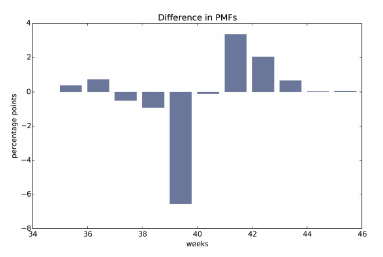
\includegraphics[scale=.70]{images/DataExplVis/pmf diff.png}
  \caption{An example of PMF difference}
  \label{fig:pmf diff}
\end{figure}

\subsection{Probability Density Function (PDF)}
The PDF is a function that describes the likelihood of a continuous 
random variable to take on a given value. It is used for continuous 
variables.

\begin{figure}[H]
  \centering
  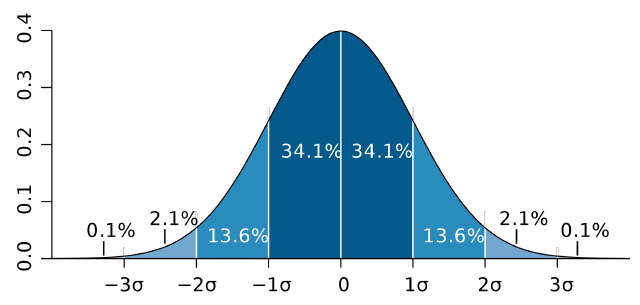
\includegraphics[scale=.60]{images/DataExplVis/pdf.png}
  \caption{An example of PDF}
  \label{fig:pdf}
\end{figure}

\subsection{Kernel Density Estimation (KDE)}
To be consistent and have better visualization we can't use the
raw histogram so with the \textbf{kernel density estimation (KDE)} we can
estimate continuous PDF based on samples.
\begin{figure}[H]
    \centering
    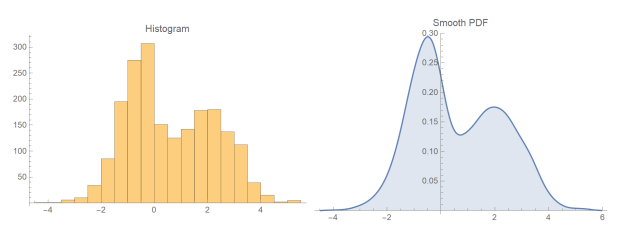
\includegraphics[scale=0.75]{images/DataExplVis/KernelDF.png}
    \caption{An histogram and its KDE}
    \label{fig:KDE}
\end{figure}
To compute that we estimate f as the \textbf{weighted average of
neighboring observed data}, where the weight is defined by the kernel
function, such that closer points are given higher weights and the
estimated function is continuous and \textit{smooth}.
\begin{center}
    $ f_{h}(x) = \frac{1}{m} \sum\limits_{i=1}^m K_{h} (x-x_{i})$
\end{center}
where $K_{h}$ is the kernel function and $h$ is the bandwidth that 
controls the smoothness of the estimated function. The most common
kernel function is the Gaussian kernel function.
\subsubsection{Effect of bandwidth}
The bandwidth is a crucial parameter in the KDE because it controls
the smoothness of the estimated function. A small bandwidth will
produce a very \textit{noisy} function, by crating false features out
of random variability, while a large bandwidth will produce a
\textit{smooth} function but with a lot of \textit{distortion}.

\subsection{Cumulative Distribution Function (CDF)}
The CDF is a function that shows the probability that a random
variables takes a value less than or equal to a given value. It is
useful to observe how the samples are distributed in different 
intervals.
$$ F(x) = P(X \leq x) = \int_{-\infty}^{x} f(x) dx$$
\begin{figure}[H]
  \centering
  \includegraphics[scale=0.60]{images/DataExplVis/CDF.png}
  \caption{An example of CDF}
  \label{fig:CDF}
\end{figure}

\subsubsection{Empirical Cumulative Distribution Function (ECDF)}
The ECDF is a \textbf{non-parametric estimator} of the CDF, that is a step 
function that jumps up by $1/n$ at each of the $n$ data points. It is 
useful to compare two or more distributions, and when the dataset is
small(CDF is heavy to compute).

\begin{figure}[H]
    \centering
    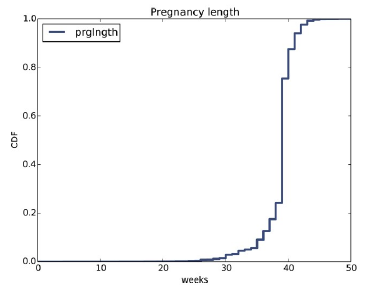
\includegraphics[scale=.80]{images/DataExplVis/ECDF.png}
    \caption{Example of ECDF}
    \label{fig:enter-label}
\end{figure}

\subsection{Percentiles and Boxplot}

Percentiles indicates the value below which given percentage of observation in a group of observation falls and similarly there is the boxplot visualization. This 2 are standardized way of displaying the distribution data based on a summary values.
The boxplot can be a little tricky and this is the various part that composed it:
\begin{itemize}
    \item median: (Q2/50th Percentile): the middle value of the attribute.
    \item first quartile (Q1/25th Percentile): the middle number between the smallest number (not the “minimum”) and the median of the attribute.
    \item third quartile (Q3/75th Percentile): the middle value between the median and the highest value (not the “maximum”) of the attribute.
    \item interquartile range (IQR): 25th to the 75th percentile.
    \item whiskers (shown in blue)
    \item \textbf{outliers} (shown as green circles)
\end{itemize}

\begin{figure}[H]
    \begin{subfigure}{.5\textwidth}
        \centering
        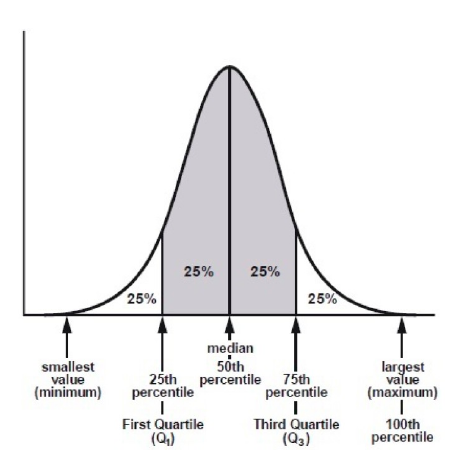
\includegraphics[width=.6\linewidth]{images/DataExplVis/Percentile.png}
        \caption{Percentile}
        \label{fig:sub1}
    \end{subfigure}
    \begin{subfigure}{.5 \textwidth}
        \centering
        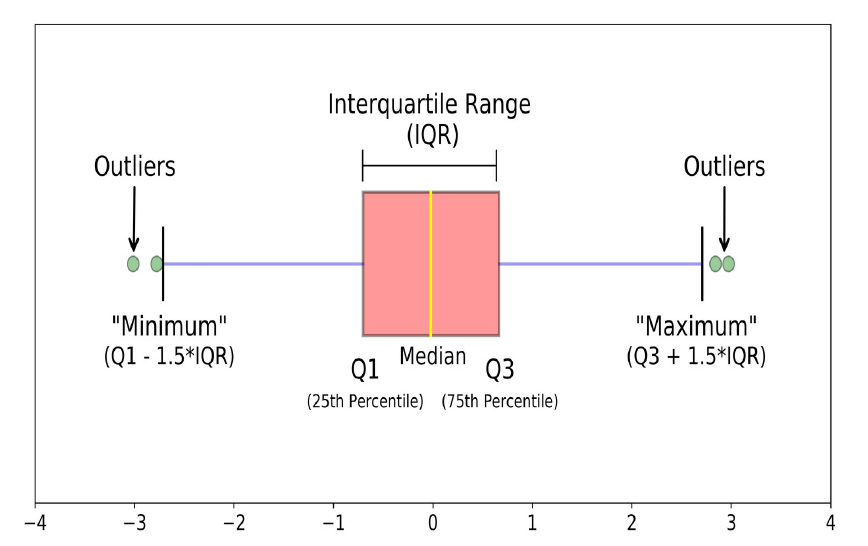
\includegraphics[width=.8\linewidth]{images/DataExplVis/Boxplot.png}
        \caption{Boxplot}
        \label{fig:sub1}
    \end{subfigure}
    \caption{Example of Percentile and Boxplot}
\end{figure}

The \textbf{Outliers} are \textit{extreme} values that might be an
errors in measurement and recording or an accurate reports of rare
events. The best way to define/handle outliers depends on “domain
knowledge” because it depends on what analysis you are planning to
address.
\subsubsection{Outliers Detection}
Outlier can be detected by \textbf{Generalized Extreme Studentized
Deviate (GESD)}, which is a statistical test that can detect one or 
more outliers in a univariate data set that follows a normal 
distribution, which is also its main limitation.
GEST performs separate test for each outlier.
\begin{equation*}
  R = \dfrac{max_{i=1,\dots,m}(|x_i - \overline{x}|)}{s}
\end{equation*}
where $x_i$ is the outlier, $\overline{s}$ is the mean of the dataset 
and $s$ is the standard deviation of the dataset.
The statistical test $R$ is recomputed recursively to remove the same 
value for the dataset(being an outlier) and the test is repeated
usepackageto the $k^{\text{th}}$ largest value.


Another method to detect is \textbf{DBSCAN} that is based on a density
clustering non-parametric algorithm. To put it simply, given a set of
points in some space, it groups together points that are closely
packed together (points with many nearby neighbors), marking as
outliers points that lie alone in low-density regions (whose nearest
neighbors are too far away)

\section{Correlation Analysis}
Datasets usually includes \textbf{different features} so the
relationship between them have a key role to describe the entire
dataset, and this is called \textbf{correlation}. This is useful
during the data exploration phase to analyse specific data
correlation because \textbf{highly correlated features} could be
\textbf{removed} simplifying the performance of data driven
algorithms.

\subsection{Scatter Plot}
The simplest way to visually check for a relationship between 2
variables is a \textbf{scatter plot}, but to have a better
comprehension of the data we have to add some \textbf{jitter}, to
introduce some noise(we alter the original values) to reverse the
effect of rounding off, as shown in figure \ref{fig:scat1}, or we can
use \textbf{transparency}(adding alpha parameter) parameters in order
to retrieve density information(darker zones correspond to higher
density) as shown in figure \ref{fig:scat2}.

\begin{figure}[H]
  \begin{subfigure}{.5\textwidth}
    \centering
    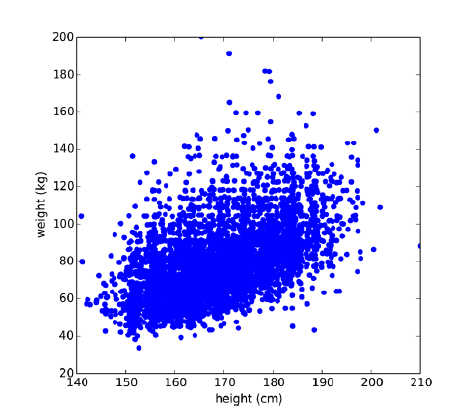
\includegraphics[width=.6\linewidth]{images/DataExplVis/Scatter1.png}
    \caption{Scatter with jitter}
    \label{fig:scat1}
  \end{subfigure}
  \begin{subfigure}{.5 \textwidth}
    \centering
    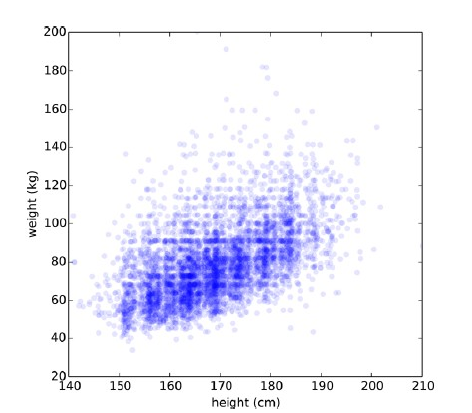
\includegraphics[width=.6\linewidth]{images/DataExplVis/Scatter2.png}
    \caption{Scatter with transparency}
    \label{fig:scat2}
  \end{subfigure}
  \caption{Example of Scatterplot}
\end{figure}

Scatterplots can be converted into \textbf{hexbin plot} that is a 
bivariate histogram useful to show the density of the data, as shown
in figure \ref{fig:hexbin}.
\begin{figure}[H]
  \centering
  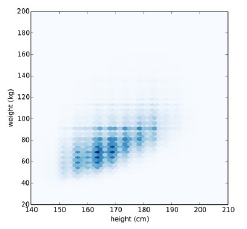
\includegraphics[scale=0.60]{images/DataExplVis/hexbin.png}
  \caption{An example of hexbin plot}
  \label{fig:hexbin}
\end{figure}

Moreover we can use scatterplot percentiles with every line that
represents one percentile to focus on the main data and not the
outlier.
\subsection{Correlation Coefficient}
A \textbf{correlation} is a statistic intended to quantify the
strength of the relationship between two variables. Possible way to
compute correlations are:
\begin{itemize}
  \item Covariance: is a measure of the joint variability of two
    random variables. In order to compare two variables, they must
    have the same unit of measurement and normalization is needed.
  \item Pearson: Solves the problem of normalization but can only
    detects linear correlation
  \item Spearman: Is a non-parametric measure of rank correlation
    that assesses how well the relationship between two variables
    can be described using a monotonic function.
\end{itemize}
The correlation, computed using the covariance, is defined as:
\begin{equation*}
  corr(x,y) = \dfrac{cov(x,y)}{std(x) \cdot std(y)}
\end{equation*}
where $cov(x,y)$ is the covariance between $x$ and $y$, $std$ is 
the standard deviation function.
We can define the covariance as:
\begin{equation*}
  cov(x,y) = \dfrac{1}{n-1} \sum_{i=1}^{n} (x_i - \overline{x}) \cdot
  (y_i - \overline{y})
\end{equation*}
where $x_i$ and $y_i$ are the values of the dataset, $\overline{x}$ 
and $\overline{y}$ are the mean of the dataset and $n$ is the number
of samples, which can be defined as:
\begin{equation*}
  \overline{x} = \dfrac{\sum_{i=1}^{n} x_i}{n}
\end{equation*}
At last, the standard deviation is defined as:
\begin{equation*}
  std(x) = \sqrt{\dfrac{1}{n} \sum_{i=1}^{n} (x_i - \overline{x})^2}
\end{equation*}



Pearson is only for linear correlation, as shown in figure
\ref{fig:pearson coff}, where you can notice that the correlation is
not linear and the cofficient is close to 0 in many cases. In this
case we can use the \textbf{Spearman correlation}, which assesses how
the relationship between two variables can be transformed into a
\textbf{rank} and described using a monotonic function.The main
advantage is that in some cases the Spearman index allows to find a
correlation when the Pearson index returns a value close to 0.
\begin{figure}[H]
  \centering
  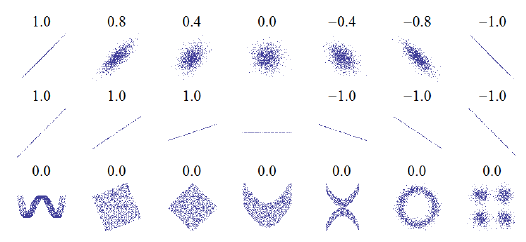
\includegraphics[scale=0.60]{images/DataExplVis/pearson coff.png}
  \caption{Some examples of non-linear correlation}
  \label{fig:pearson coff}
\end{figure}
For a sample of size $m$, the $m$ raw scores $x_i$ and $y_i$ are
converted to ranks $R(x_i)$ and $R(y_i)$, and the Spearman correlation 
coefficient is computed as:
\begin{equation*}
  r_s = \rho(R(x), R(y)) = \dfrac{cov(R(x), R(y))}{\sigma_{R(x)} \cdot 
  \sigma_{R(y)}}
\end{equation*}
but if all the $m$ ranks are \textbf{distinct integers}, the Spearman
correlation coefficient can be computed as: 
\begin{equation*}
  r_s = 1 - \dfrac{6 \sum_{i=1}^{m} d_i^2}{m(m^2 - 1)}
\end{equation*}
where $d_i = R(x_i) - R(y_i)$ is the difference between the ranks of 
the two variables.

Spearman correlation is 
\begin{itemize}
  \item 1 when two variables are perfectly monotonically related
  \item -1 when two variables are perfectly inversely monotonically
    related
  \item 0 when there is no monotonic relationship between the two
    variables
\end{itemize}

As a rule of thumb, to compute the coefficients we can use the following 
method:
\begin{enumerate}
  \item \textbf{Rank} the two \textbf{data sets}. Ranking is achieved
    by giving the ranking '1' to the biggest number in a column, '2'
    to the second biggest value and so on. The smallest value in the
    column will get the lowest ranking.
  \item Tied scores are given the mean (average) rank. For example, if
    there are three tied scores ranked fifth (fifth, sixth and
    seventh), the mean rank in this case is calculated as $(5+6+7)/3 =
    6$.
  \item \textbf{Calculate the difference} between the two ranks for 
    each data point. For example, if the rank of data point 1 in data
    set 1 is 3 and its rank in data set 2 is 4, the difference is 1.
  \item use the formula to calculate the correlation coefficient.
\end{enumerate}


\section{Other Data Visualization}
Other data visualization are:
\begin{itemize}
  \item \textbf{Heatmap}, the visualization of a correlation
    matrix(figure \ref{fig:sub1})
  \item \textbf{Word Cloud}, a visual representation of text data in
    which the size of each word indicates its frequency or importance
    (figure \ref{fig:sub1})
  \item \textbf{PCA}, a technique to reduce the dimensionality of the
    data by projecting it into a lower-dimensional space (figure
    \ref{fig:sub1})
  \item \textbf{T-SNE}, a technique to reduce the dimensionality of
    the data by projecting it into a lower-dimensional space (figure
    \ref{fig:sub1})
\end{itemize}

%4 figures  2x2
\begin{figure}[H]
    \begin{subfigure}{.5\textwidth}
        \centering
        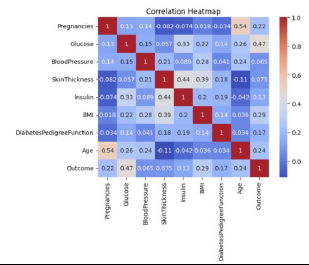
\includegraphics[width=.6\linewidth]{images/DataExplVis/heatmap.png}
        \caption{Heatmap}
        \label{fig:sub1}
    \end{subfigure}
    \begin{subfigure}{.5 \textwidth}
        \centering
        \includegraphics[width=.8\linewidth]{images/DataExplVis/word
        cloud.png}
        \caption{Word Cloud}
        \label{fig:sub1}
    \end{subfigure}
    \begin{subfigure}{.5 \textwidth}
        \centering
        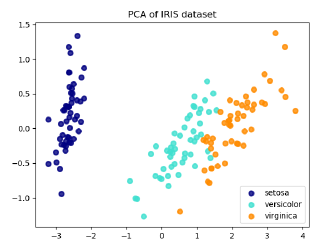
\includegraphics[width=.8\linewidth]{images/DataExplVis/pca.png}
        \caption{PCA}
        \label{fig:sub1}
    \end{subfigure}
    \begin{subfigure}{.5 \textwidth}
        \centering
        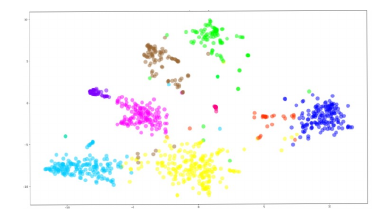
\includegraphics[width=.8\linewidth]{images/DataExplVis/t-sne.png}
        \caption{T-SNE}
        \label{fig:sub1}
    \end{subfigure}
    \caption{Other Data Visualization}
  \end{figure}

    



